% !Mode:: "TeX:UTF-8"
%!TEX program  = xelatex

\documentclass{cumcmthesis}
%\documentclass[withoutpreface,bwprint]{cumcmthesis} %去掉封面与编号页

\usepackage{url}
\usepackage{enumerate}
\title{(2018B)智能RGV的动态调度策略}
\tihao{B}
\baominghao{01001015}
\schoolname{北京大学}
\membera{包慧语}
\memberb{孟逸白}
\memberc{吴越}
\supervisor{}
\yearinput{2018}
\monthinput{09}
\dayinput{16}

\begin{document}

\maketitle
\begin{abstract}

本文是对智能 RGV的动态调度策略问题的研究。我们对原问题建模并设计算法,然后在写好的模拟器代码上实现算法来求得在该算法下此智能RGV可以完成多少产品的加工任务。

第一种情况中,我们首先通过尝试了一种贪心的算法来求得答案,随后又使用了三层的深度优先搜索来决策,对这两种结果进行比较,评估一下算法的优劣。

第二种情况中,我们采用了类似的贪心策略,通过穷举加工第一道工序的CNC和加工第二道工序的CNC的排布方法,来选取可以加工最多的产品的排布,并利用设计的算法来模拟产品的加工,求得最后的答案。

第三种情况中,问题带有随机性。在前两问里,机器的行为是可以预测的,我们知道送给CNC的产品什么时候可以加工好,于是我们可以根据这一信息来进行决策,来决定RGV下一步的行动。而第三问则有一个随机的过程,机器在加工的过程中会有$1\%$的概率出现故障。对于只有一种工序的情况,我们运行20次取最后的平均值,来求得最后的答案,检验我们的算法有效性。对于两道工序的情况,我们同样穷举加工第一道工序的CNC和加工第二道工序的CNC的排布方法,然后运行20次取平均值,来选取平均意义下最优的排布方式,来解决这个问题。

\keywords{调度算法\quad  随机过程\quad   贪心策略\quad  穷举搜索}
\end{abstract}

%目录
%\tableofcontents

\section{问题重述}

一个智能加工系统由8台计算机数控机床(Computer Number Controller,CNC)、1辆轨道式自动引导车(Rail Guide Vehicle,RGV)、1条RGV直线轨道、1条上料传送带、1条下料传送带等附属设备组成。RGV是一种无人驾驶、能在固定轨道上自由运行的智能车。它根据指令能自动控制移动方向和距离,并自带一个机械手臂、两只机械手爪和物料清洗槽,能够完成上下料及清洗物料等作业任务。

\subsection{对各部件的详细解释}

\begin{enumerate}[(1)]

\item CNC:在上料传送带和下料传送带的两侧各安装4台CNC,等距排列,每台CNC同一时间只能安装1种刀具加工1个物料。如果物料的加工过程需要两道工序,则需要有不同的CNC安装不同的刀具分别加工完成,在加工过程中不能更换刀具。第一和第二道工序需要在不同的CNC上依次加工完成,完成时间也不同,每台CNC只能完成其中的一道工序。

\item RGV:RGV带有智能控制功能,能够接收和发送指令信号。根据指令能在直线轨道上移动和停止等待,可连续移动1个单位(两台相邻CNC间的距离)、2个单位(三台相邻CNC间的距离)和3个单位(四台相邻CNC间的距离)。RGV同一时间只能执行移动、停止等待、上下料和清洗作业中的一项。

\item 上料传送带:上料传送带由4段组成,在奇数编号CNC1\#、3\#、5\#、7\#前各有1段。由系统传感器控制,只能向一个方向传动,既能连动,也能独立运动。

\item 下料传送带:下料传送带由4段组成,在偶数编号CNC2\#、4\#、6\#、8\#前各有1段。由传感器控制,只能向同一个方向传动,既能连动,也能独立运动。

\end{enumerate}

\subsection{作业流程}

\begin{enumerate}[(1)]
	
\item 智能加工系统通电启动后,RGV在CNC1\#和CNC2\#正中间的初始位置,所有CNC都处于空闲状态。

\item 在工作正常情况下,如果某CNC处于空闲状态,则向RGV发出上料需求信号;否则,CNC处于加工作业状态,在加工作业完成即刻向RGV发出需求信号。

\item RGV在收到某CNC的需求信号后,它会自行确定该CNC的上下料作业次序,并依次按顺序为其上下料作业。根据需求指令,RGV运行至需要作业的某CNC处,同时上料传送带将生料送到该CNC正前方,供RGV上料作业。RGV为偶数编号CNC一次上下料所需时间要大于为奇数编号CNC一次上下料所需时间。

\item 在RGV为某CNC完成一次上下料作业后,就会转动机械臂,将一只机械手上的熟料移动到清洗槽上方,进行清洗作业(只清洗加工完成的熟料)。具体过程:首先用另一只机械手抓取出清洗槽中的成料、转动手爪、放入熟料到清洗槽中,然后转动机械臂,将成料放到下料传送带上送出系统。这个作业过程所需要的时间称为RGV清洗作业时间,并且在这个过程中RGV不能移动。熟料在清洗槽中的实际清洗时间是很短的,远小于机械手将成料放到下料传送带上的时间。

\item RGV在完成一项作业任务后,立即判别执行下一个作业指令。此时,如果没有接到其他的作业指令,则RGV就在原地等待直到下一个作业指令。某CNC完成一个物料的加工作业任务后,即刻向RGV发出需求信号。如果RGV没能即刻到达为其上下料,该CNC就会出现等待。

\item 系统周而复始地重复(3)至(5),直到系统停止作业,RGV回到初始位置。

\end{enumerate}

\subsection{三种情况的问题}

而我们的任务是建立数学模型和算法,来解决以下三种情况的问题:

\begin{enumerate}[(1)]
	
\item 一道工序的物料加工作业情况,每台CNC安装同样的刀具,物料可以在任一台CNC上加工完成;
\item 两道工序的物料加工作业情况,每个物料的第一和第二道工序分别由两台不同的CNC依次加工完成;
\item CNC在加工过程中可能发生故障(据统计:故障的发生概率约为1\%)的情况,每次故障排除(人工处理,未完成的物料报废)时间介于10~20分钟之间,故障排除后即刻加入作业序列。要求分别考虑一道工序和两道工序的物料加工作业情况。

\end{enumerate}

对于一般的问题,我们需要建立模型提出算法,然后代入提供的三组数据,给出真实的调度策略以及系统的工作效率。

\subsection{问题的分析}

\subsubsection{第一种情况的分析}

为了能够加工完更多的产品,那么我们的想法就是让所有CNC的总等待时间尽量小。为了达到这一目的,我们会对8个CNC最早可以开始工作的时间进行排序,让RGV前往最早可以开始工作的CNC,这样不断循环直到时间结束。我们利用这样的一个贪心的策略来编写算法。我们实现了另外一个版本,是利用三层的深度优先搜索来决策下一步RGV需要去哪里。

\subsubsection{第二种情况的分析}

同样为了加工完成更多的产品,我们的想法也是先找一个最快可以开始工作的地方,分CNC加工的是第几道工序区别来运行不同的后续逻辑。同样也是利用一个贪心的策略来进行决策,运行程序,检验算法的有效性。

\subsubsection{第三种情况的分析}

第三种情况比前两种情况多了一个事件:机器会有1\%的概率发生故障。我们在前两种情况的算法基础上增加了一个随机数变量,使得运行中的机器有1\%的概率发生错误,同时产生另外一个随机数,表示机器修好的时间。而在决策过程中,我们会自动忽略所有故障中的机器。其余的决策过程和前两种情况类似。对于这样一个随机的过程,我们会运行20次取平均值,来求得一个接近期望的数值,表示我们算法的结果。


\section{模型的假设}

\begin{itemize}
\item 对于第一问和第二问,所有的时间可预测,决策可以使用未来的信息进行推断
\item 在第三问中机器的损坏是随机并且不可预测的,所以决策系统只知道此机器损坏的消息,同时不知道什么时候能够修好
\item 对于系统的作业效率,我们的理解是CNC真正在工作的时间除以CNC总共可以工作的时间
\end{itemize}

\section{符号说明}
\begin{center}
\begin{tabular}{cc}
 \hline
 \makebox[0.3\textwidth][c]{符号}	&  \makebox[0.4\textwidth][c]{意义} \\ \hline
 s	    	& 生产环境模拟器对象     	 \\ \hline
 s.cnc	    & 生产环境中的cnc机器列表 	\\ \hline
 s.rgv      & RGV轨道式自动引导车 		  \\ \hline
 s.time		& 模拟器的当前时间			  \\ \hline
 s.objs		& 已经完成的工件对象列表	   \\ \hline
 s.errs		& 发生的错误记录列表			 \\ \hline
 s.err\_rate& 错误发生率					\\ \hline
 
\end{tabular}
\end{center}

\section{算法详解}

\subsection{情况一算法}

如前述,我们先自己实现了一个智能加工系统的模拟器(simulator.py),可以模拟进行上下料、清洗、RGV移动等各种操作。随后我们先实现了一个贪心算法(choose1.py)。算法的主要思想是我们对8个CNC最早可以开始工作的时间进行排序。对于每个CNC,它最早可以开始工作的时间指的是RGV移动到它之后的时间与他结束自身工作的时间中的较大值,也就是代码中的 max(walk\_finish,s.Cnc(i).finish\_time())。我们取8个CNC中最早可以开始工作的一个,开始工作。如此循环一直到时间结束。我们运行代码并获得了3组参数下该系统的实际调度策略以及系统的作业效率,调度策略在支撑材料中,而作业效率如下表所示。

\begin{table}[!htbp]
\caption{单工序无故障的作业效率} \centering
\begin{tabular}{cccc}
\hline
&第一组参数&第二组参数&第三组参数\\
\hline
作业效率&92.85\%&90.37\%&92.73\%\\
\hline
\end{tabular}
\end{table}
	
经过对数据的分析可知:对于单工序的情况,我们的算法效率还是较高的,对于三组数据都有90\%以上的作业效率。这说明利用贪心的策略可以使CNC有较高的利用率,我们的策略是较为成功的。

同样我们也实现了三层深度优先搜索的算法(choose1bru.py)。这个算法的想法是我们穷举RGV的之后三步走动与上下料,容易知道我们的搜索空间是一个深度为3的八叉树,我们选择时间最短的一个分支,向下走一步,然后继续进行深搜。通过对三组实际数据进行实验,我们发现最后的结果与我们贪心策略的结果是一致的,于是实验结果我们在此省略。

%问题流程图:
%\begin{figure}[!h]
%\centering
%\caption{问题三流程图}
%\end{figure}

\subsection{情况二算法}

对于第二种情况,我们同样采用了一个类似的贪心算法(choose2.py)。我们穷举加工第一道工序的CNC和加工第二道工序的CNC的排布方法,对每种排布方法,我们采用如下的贪心策略来进行决策:我们同样是对每个CNC最快可以开始工作的时间进行排序,然后我们选取一个最快可以开始工作的CNC(空闲状态的加工第二道工序的CNC除外),让RGV前往该处。如果这是处理第一道工序的CNC,在上料后RGV 查看一下是否获取了一个半成品,如果是,那么此时RGV就要前往最快可以开始工作的加工第二道工序的CNC,让其加工该半成品,此时如果拿到成品则进行清洗工作;如果RGV 并没有获取半成品,那么这一次循环结束,重新寻找下一个最快可以开始工作的CNC。如果一开始选取的是加工第二道工序的CNC,那么RGV就会直接下料,并进行清洗,这一次循环结束。

我们的主要想法就是让RGV前往可以尽快开始工作的地方,需要注意之处就是在于当RGV拿到半成品之后,由于RGV的手的数量有限,只能去前往加工第二道工序的CNC,而不是在全局搜索一个可以最快开始工作的地方。

经过对三组实际数据的运行,我们得到了如下的作业效率:

\begin{table}[!htbp]
\caption{双工序无故障的作业效率} \centering
\begin{tabular}{cccc}
\hline
&第一组参数&第二组参数&第三组参数\\
\hline
作业效率&85.47\%&71.49\%&66.40\%\\
\hline
\end{tabular}
\end{table}

经过对数据的分析可知对于第一组参数来说,我们的算法表现较好。经分析可知,由于第一组数据中第一道以及第二道加工工序的时间相近,我们可以得到一个较高的效率。而当两道工序的加工时间差距较大时,就可能会产生一些空闲时间。第二组参数的第二道工序时间长,就会有许多只加工完第一道工序的产品处于等待中,等待加工第二道工序的CNC有空闲。第三组参数的第一道工序时间长,就会有许多加工完第二道工序的CNC处于等待中,等待其他CNC加工好的半成品。所以说对于后两组参数,作业效率必然不会太高,而我们的程序给出了大约70\%的加工效率,也是一个不错的结果。

\subsection{情况三算法}

对于可能出现故障的机器,我们只需要对我们的算法略做修改即可。对于任意一台CNC,当元件被送入机器后,机器都有1\%的概率出现故障。在机器的修复过程中,我们的算法认为该台机器并不存在,而在故障修复后,该机器会立刻加入我们的考察队列中。我们以此来模拟出现故障的机器。而由于一次过程中存在随机性,我们会对每种情况都运行20次取平均值。在只有一道工序的时候,我们认为这个平均值就是我们算法求得的加工产品数量。在有两道工序的时候,我们穷举加工第一道工序的CNC和加工第二道工序的CNC的排布方法,对每种方法都运行20次求得平均加工数量,然后我们采用平均值最高的一种CNC排布方案当作我们选择的方案。

通过在三组实际数据上进行试验,我们得到了加工的调度策略(见支撑材料)以及作业效率(如下表):

\begin{table}[!htbp]
\caption{单工序有故障的作业效率} \centering
\begin{tabular}{cccc}
\hline
&第一组参数&第二组参数&第三组参数\\
\hline
作业效率&90.56\%&88.06\%&89.97\%\\
\hline
\end{tabular}
\end{table}

\begin{table}[!htbp]
\caption{双工序有故障的作业效率} \centering
\begin{tabular}{cccc}
\hline
&第一组参数&第二组参数&第三组参数\\
\hline
作业效率&79.56\%&68.42\%&62.75\%\\
\hline
\end{tabular}
\end{table}

经过对数据的分析可知,即使存在着潜在的故障问题,单工序时的系统作业效率也是极其优异的,都在90\%附近。这和没有故障时的效率相仿,这也说明了我们的算法是可以信赖的。而在双工序的情况下,我们的作业效率有着微小的下滑,这是难免的。因为若在加工过程中产生故障,将会浪费很多时间,进而拖低我们的效率。我们认为效率下滑的最主要因素即是潜在会出现的故障。总之,我们的算法在有故障存在的同时也给出了较为优秀的表现,这充分说明了我们的模型是实用的,算法是有效的。

\section{随机模型评估}

题目中给定错误的发生概率为1\%,但是由模拟器的实际测试情况,大约完成300~400个零件,如果按照1\%的概率计算,只有3~4个零件。为了验证此数据的波动,我们尝试模拟加工1000000次400个工件的过程,获得损坏个数的分布,如下图

\begin{center}
	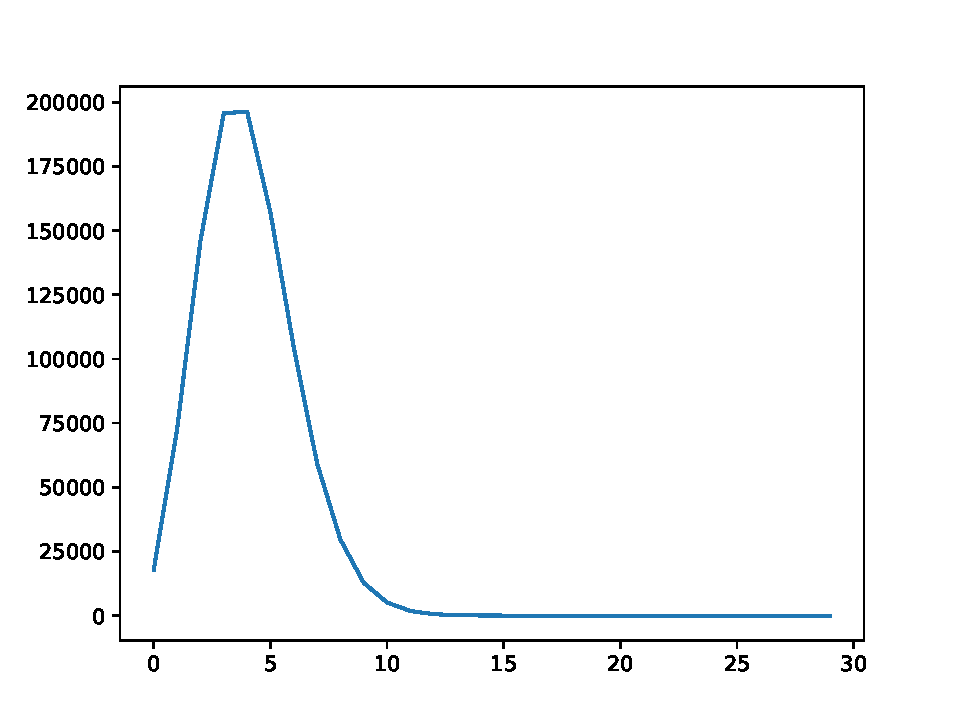
\includegraphics[scale=0.6]{random_distribution.pdf}
\end{center}

可以看出,除了损坏刚好1\%,即4个工件,在附近都有不小的分布,这说明对于我们算法的衡量需要进行大量的实验才能说明其性能。

对于第三题的第一小问,我们尝试使用第一组参数,测试200000次得到如下图的分布

\begin{center}
	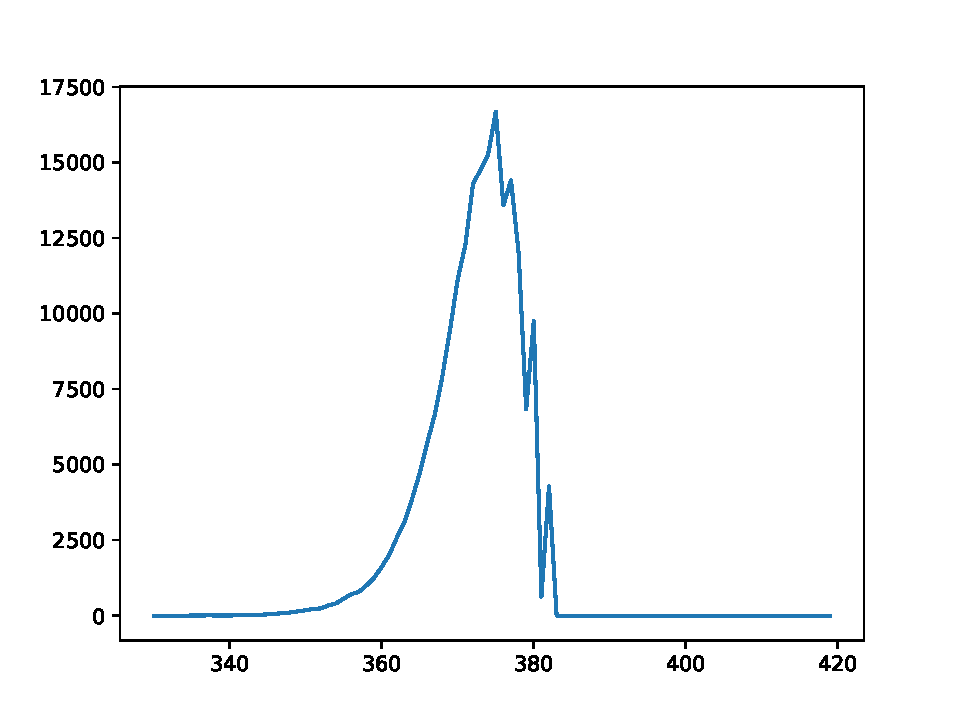
\includegraphics[scale=0.6]{case31_distribution.pdf}
\end{center}

\section{总结}

本文利用了贪心策略和深度优先搜索策略,对于原问题建立起的模型给出了较好的结果。我们的目的就是让RGV的空闲时间尽量少,所以我们希望RGV总是能够前往较快能开始工作的地方。

\subsection{模型优点}

1、实现了一个完全的智能加工系统模拟器(simulator.py),该框架的存在使得我们的程序编写十分方便,可以应用各种算法。

2、使用了贪心以及深度优先算法对其中一个问题比较,得到了一定的结论。

\subsection{模型缺点}

1、对于两道工序的情况,穷举排布情况耗时长。

2、机器的使用效率不够高,希望可以利用启发式搜索来增加效率。

%参考文献
\begin{thebibliography}{9}%宽度9
\bibitem{bib:one} 司守奎,孙玺菁. 数学建模算法与应用 [M]. 北京,国防工业出版社,2011
\bibitem{bib:two} 姜启源,谢金星等. 数学建模(第四版)[M].北京:高等教育出版社,2011.
\end{thebibliography}

\newpage
%附录
\begin{appendices}
\section{RGV行为模拟器--Python源代码}
\lstinputlisting[language=python]{../simulator.py}
\section{第一题决策器--Python源代码}
\lstinputlisting[language=python]{../choose1.py}
\section{第二题决策器--Python源代码}
\lstinputlisting[language=python]{../choose2.py}
\section{第三题(1)决策器--Python源代码}
\lstinputlisting[language=python]{../choose31.py}
\section{第三题(2)决策器--Python源代码}
\lstinputlisting[language=python]{../choose32.py}
\section{结果生成器--Python源代码}
\lstinputlisting[language=python]{../write_excel.py}


\end{appendices}

\end{document}
